\section{SequenceViewer}\label{sec:sequenceviewer}
The GIRAF multiproject contains three applications which share a common feature, which is sequences of pictograms. The three applications are Sekvens, Livshistorier, and Piktooplæser. During sprint 2, these three groups held a meeting regarding a common need for storing sequences in the database. During this meeting, a new project was established, namely Sequenceviewer. The Seqeuenceviewer was decided to be a front-end application, which the three other applications should call whenever they want to display a sequence to a child. This new application should ensure a common interface whenever the children interact with the system. The sequences of pictograms will be displayed in the same way, whichever application the guardians previously used to make a sequence of pictograms.
The purpose of Sequenceviewer is to act as a service to the three other applications. It is not suppose to be apparent to the guardians or the children, that they actually enter the Sequenceviewer application. The position of Sequenceviewer in the GIRAF multiproject is shown in figure \ref{fig:sequenceviewer}.
\begin{figure}[H]
	\centering
	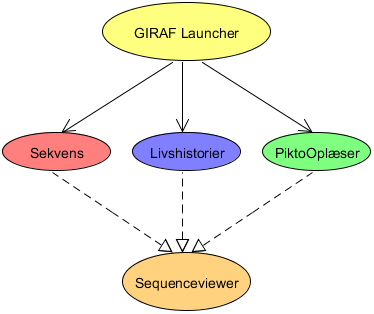
\includegraphics[scale=0.8]{Pics/sequenceviewer}
	\caption{The position of Sequenceviewer in the GIRAF multiproject.}
	\label{fig:sequenceviewer}
\end{figure}
The stippled lines between the three applications and Sequenceviewer, represent the fact that it should not be apparent to the users that they enter Sequenceviewer.

Here are the requirements to Sequenceviewer, these became clear during the meeting:
\begin{itemize}
\item It should be able to show a choice between 2 or more pictograms. Choosing a pictogram should now take the place in the sequence, which before held the choice-pictogram.
\note{Add some pictures for this functionality please}
\item It should be able to show nested sequences, meaning that a pictogram in a sequence can also be a whole sequence. When a child presses the sequence it should open the sequence related to it.
\item It should be able to mark a pictogram as "done" by highlighting or moving an arrow-marker.
\item It should show a sequence of pictograms up to 7 at a time. This should be adjustable in a settings menu for each of the applications before Sequenceviewer is opened.
\item It should be able to be display a sequence in landscape- or portrait-mode. This should also be a choice in a settings activity.
\item It should be able to exit Sequenceviewer and return to the previous activity.
\item It should not show pictograms in the sequence with cut edges or even half pictograms.
\end{itemize}